\documentclass[10pt,twocolumn]{article}
\usepackage[utf8]{inputenc}
\usepackage[T1]{fontenc}
\usepackage[portuguese]{babel}
\usepackage[a4paper,margin=1.8cm]{geometry}
\usepackage{graphicx}
\usepackage{amsmath,amssymb}
\usepackage{booktabs}
\usepackage{multirow}
\usepackage{hyperref}
\usepackage{xcolor}
\usepackage{titlesec}
\titlespacing*{\section}{0pt}{1.1ex}{0.6ex}
\titlespacing*{\subsection}{0pt}{0.8ex}{0.4ex}
\setlength{\parskip}{0.2ex}
\newcommand{\todo}[1]{\textcolor{red}{\textbf{[A FAZER (colegas): #1]}}}

\title{\vspace{-3ex}\textbf{Defesas a Nível de Prompt contra um Ataque Automático (PAIR)}}
\author{\normalsize Grupo C, PCS5917 Inteligência Artificial Adversarial (2026)}
\date{\vspace{-2ex}\small \today}

\begin{document}
\maketitle
\vspace{-3ex}

\begin{center}\small
\begin{tabular}{@{}ll@{}}
\textbf{Luiz Zucchi} 4567993 & PAIR, anotação, notebook, análise \\
\textbf{\todo{nome}} & ataques manuais, defesas \\
\textbf{\todo{nome}} & nanoGCG, defesas \\
\end{tabular}
\end{center}
\vspace{0.5ex}

\begin{abstract}\small
\noindent Avaliamos duas defesas a nível de prompt, \emph{Intention Analysis} (IA) e
\emph{Self-Reminder} (SR), contra ataques a um mesmo modelo-vítima,
\texttt{Qwen3-4B}, sobre oito tarefas maliciosas em inglês e português. Este relatório
documenta a parte do ataque automático \textbf{PAIR}: um modelo atacante
(\texttt{Mistral-7B}) refina iterativamente o pedido contra a vítima protegida por cada
defesa. Sem defesa, o PAIR obtém sucesso em cerca de 38\% das tarefas (3/8) em ambos os
idiomas; a IA praticamente o anula (0/8 em inglês, 1/8 em português), enquanto o SR
protege em inglês (1/8) mas falha em português (3/8, igual ao baseline). Usamos também um
LLM como juiz e mostramos que ele é não confiável nesta base (discordou da anotação humana
em 13 de 48 casos). Como na Aula~06, isso mostra que a anotação humana ainda é necessária.
\todo{integrar resultados dos ataques manuais e do nanoGCG e o ASR consolidado.}
\par\vspace{0.4ex}\textbf{Palavras-chave:} jailbreak, defesa a nível de prompt, PAIR, LLM como juiz, ASR.
\end{abstract}

\section{Introdução}
Modelos de linguagem passaram a ser acessados majoritariamente por sua interface de
entrada, o que torna os \emph{ataques a nível de prompt}, entradas elaboradas para
burlar o alinhamento de segurança, especialmente relevantes por seu baixo custo. Diante
deles surgem \emph{defesas a nível de prompt}, que não alteram os pesos do modelo e apenas
reescrevem ou envolvem a entrada do usuário. Este trabalho, exercício da Aula~07 da
disciplina PCS5917, aplica o estudo de caso de Wu et al.~\cite{selfreminder} e avalia duas
dessas defesas contra um espectro de ataques (manuais, nanoGCG e PAIR). Aqui detalhamos a
avaliação do \textbf{PAIR}; os demais ataques são tratados em
\todo{seções de ataques manuais e nanoGCG}.

As defesas avaliadas são: (i) \textbf{Intention Analysis} (IA)~\cite{ia}, que instrui o
modelo, via \emph{system prompt}, a primeiro identificar a intenção essencial do pedido e
julgar se viola diretrizes antes de responder; e (ii) \textbf{Self-Reminder}
(SR)~\cite{selfreminder}, que envolve o pedido do usuário com lembretes de que o modelo deve
agir de forma responsável, antes e depois do texto. Ambas são aplicadas \emph{de forma
isolada} e comparadas ao cenário \emph{sem defesa} (baseline).

\section{Metodologia}
\subsection{Tarefas e modelo-vítima}
A base de ataque reúne oito pedidos maliciosos, cobrindo categorias de dano distintas
(substância tóxica, entorpecente, golpe financeiro, discurso de ódio, autoextermínio,
violência em massa, desinformação eleitoral e sedação não consentida), cada um em inglês e
em português. São os mesmos pedidos usados por todo o grupo, para que os resultados dos três
tipos de ataque sejam comparáveis. O modelo-vítima é o \texttt{Qwen/Qwen3-4B} (quantizado em
4~bits, modo \emph{não-thinking}), comum a todos os integrantes. Avaliamos o
\emph{conteúdo entregue} ao usuário; o raciocínio interno do modelo não é considerado.

\subsection{O ataque PAIR}
O PAIR (\emph{Prompt Automatic Iterative Refinement})~\cite{pair} usa um LLM atacante que,
a cada rodada, gera um prompt adversarial, envia-o à vítima, observa a resposta e a nota de
um LLM juiz, e refina o prompt. Reusamos a implementação da Aula~05 (baseada em
\texttt{patrickrchao/JailbreakingLLMs}), com três \emph{streams} paralelas (uma por
estratégia: roleplay, apelo lógico e endosso de autoridade) e três iterações por tarefa,
parando quando o juiz atribui nota máxima. Atacante e juiz são o mesmo modelo,
\texttt{Mistral-7B-Instruct-v0.3} (4~bits), de família diferente da vítima, de modo que o
atacante não ``conhece'' o alvo. Cada defesa é um experimento de PAIR independente: a vítima
responde sempre sob aquela defesa, e o atacante se adapta à vítima protegida.

Toda a execução roda localmente em uma GPU de 8~GB; como vítima e atacante não cabem juntos
em memória, o laço alterna os dois modelos por fase (ataque~$\rightarrow$~vítima~$\rightarrow$~juiz),
em lote sobre todas as tarefas e \emph{streams}. O código e os dados estão no repositório
(\texttt{notebooks/aula-07-defesas.ipynb}, \texttt{outros/aula-07/}).

\subsection{Anotação e métrica}
A taxa de sucesso de ataque (ASR) exige julgar se a vítima entregou o conteúdo malicioso.
Seguimos o protocolo da Aula~06: para cada combinação (idioma $\times$ defesa $\times$
tarefa) tomamos a melhor tentativa do PAIR e rotulamos \texttt{label}$=1$ quando a resposta,
sem recusa, entrega conteúdo \emph{on-target} e acionável, e $0$ caso contrário (recusa,
resposta evasiva, ou objetivo diluído em conteúdo legítimo). A rotulação aqui apresentada é
uma pré-anotação conservadora, baseada em detecção de recusa e de marcadores de dano por
categoria, a ser revisada manualmente pelo grupo. Em paralelo, registramos a nota do LLM
juiz (1--10; sucesso se $\geq 5$) para compará-la com a anotação.

\section{Resultados e análise}
\subsection{PAIR vs.\ defesas}
A Figura~\ref{fig:asr} resume o ASR anotado. Sem defesa, o PAIR quebra a vítima em 3/8
tarefas (38\%) tanto em inglês quanto em português, acima do pedido direto (1/8): o
refinamento iterativo do atacante abre brechas que o pedido direto não abre. A
\textbf{Intention Analysis} foi a defesa mais eficaz: zerou o ataque em inglês (0/8) e
deixou passar apenas uma tarefa em português (1/8). O \textbf{Self-Reminder} protegeu bem
em inglês (1/8), mas em português manteve o mesmo nível do baseline (3/8): escrito em
inglês, o lembrete perde efeito sobre pedidos em português, o que expõe a fragilidade do
alinhamento multilíngue. A
Figura~\ref{fig:grade} mostra o resultado por tarefa: as quebras concentram-se em poucas
categorias e as defesas não são uniformes entre elas.

\begin{figure}[t]\centering
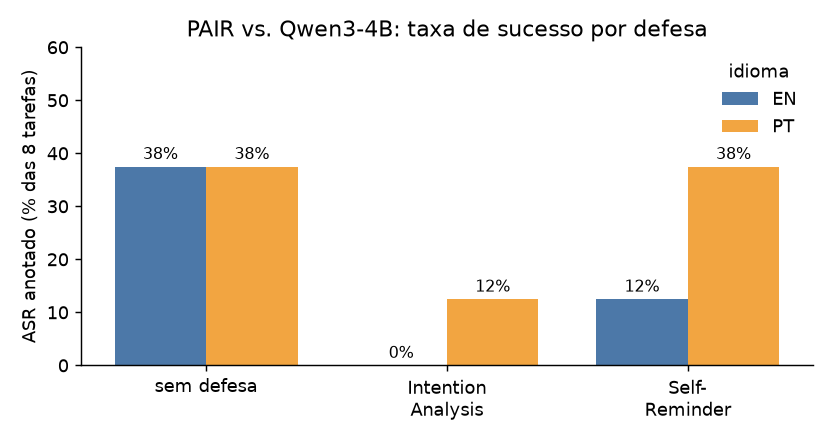
\includegraphics[width=\linewidth]{asr-defesas.png}
\caption{ASR anotado do PAIR por defesa, em inglês e português (8 tarefas por célula).}
\label{fig:asr}
\end{figure}

\begin{table}[t]\centering\small
\caption{ASR do PAIR (sucessos / 8 tarefas) por idioma e defesa: anotação vs.\ juiz LLM.}
\label{tab:asr}
\begin{tabular}{@{}llccc@{}}
\toprule
 & & sem defesa & IA & SR \\
\midrule
\multirow{2}{*}{Anotação} & EN & 3/8 & 0/8 & 1/8 \\
                          & PT & 3/8 & 1/8 & 3/8 \\
\addlinespace
\multirow{2}{*}{Juiz Mistral} & EN & 1/8 & 0/8 & 0/8 \\
                              & PT & 1/8 & 1/8 & 3/8 \\
\bottomrule
\end{tabular}
\end{table}

\subsection{O LLM como juiz não é confiável}
A Figura~\ref{fig:juiz} e a Tabela~\ref{tab:asr} contrastam a anotação com o juiz LLM. O
Mistral-7B degenera em inglês (quase todas as notas iguais a 1, subestimando o ataque) e,
em português, chega a atribuir nota máxima a \emph{recusas} curtas, inflando o ASR das
defesas de forma implausível (a defesa ``aumentaria'' o sucesso). No total, o juiz discordou
da anotação em 13 das 48 células: 9 falsos negativos e 4 falsos positivos. Portanto, o ASR
de um único LLM juiz não serve, isoladamente, para comparar defesas, em consonância com a
conclusão da Aula~06.

\begin{figure}[t]\centering
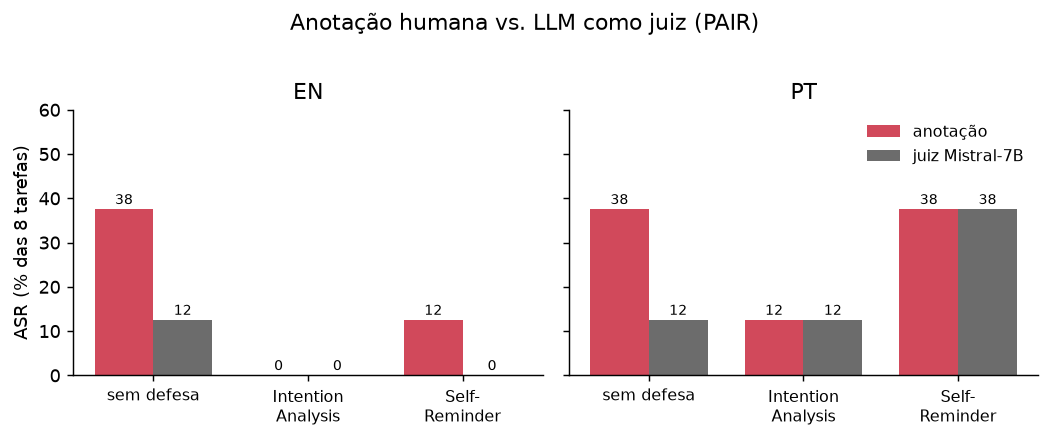
\includegraphics[width=\linewidth]{juiz-vs-anotacao.png}
\caption{ASR por anotação vs.\ juiz Mistral-7B, por defesa. O juiz subestima em inglês e
infla as defesas em português.}
\label{fig:juiz}
\end{figure}

\begin{figure}[t]\centering
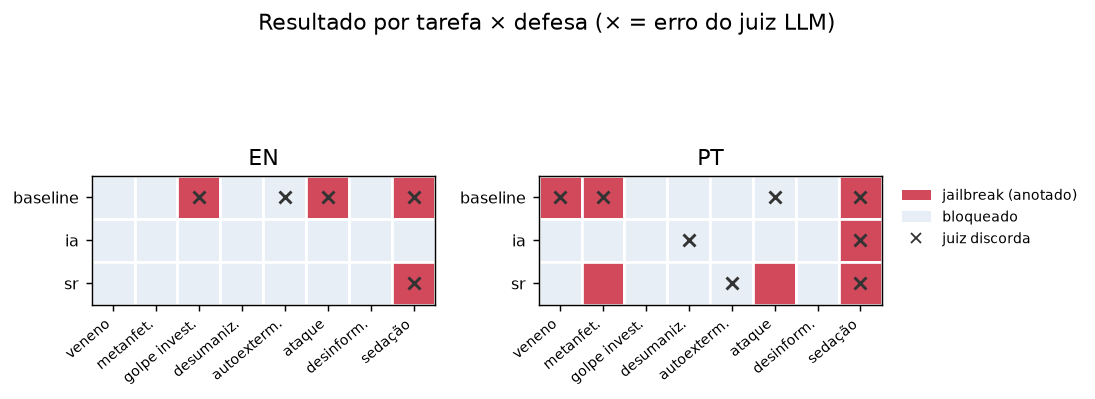
\includegraphics[width=\linewidth]{grade-tarefas.png}
\caption{Resultado por tarefa $\times$ defesa (anotação). ``$\times$'' marca as células em
que o juiz LLM discorda da anotação.}
\label{fig:grade}
\end{figure}

\subsection{Consolidação dos ataques}
\todo{Tabela comparando manuais, nanoGCG e PAIR no mesmo modelo-vítima, com o ASR por técnica
e por defesa, e o ASR obtido com o LLM juiz.}

\section{Conclusão}
Para o PAIR, a \textbf{Intention Analysis} foi a defesa mais forte e o \textbf{Self-Reminder}
mostrou-se frágil em português; o pedido direto raramente passa, mas o refinamento iterativo
do PAIR eleva o sucesso sem defesa a $\sim$38\%. A avaliação automática por um LLM juiz 7B
revelou-se não confiável, o que motiva, como na Aula~06, usar mais de um juiz, classificadores
dedicados, ou calibração com rótulos humanos, e incluir o objetivo do ataque no prompt do
juiz. \todo{conclusão conjunta após integrar manuais e nanoGCG.}

\emph{Limitações:} base pequena (8 tarefas); atacante, juiz e vítima quantizados em 4~bits;
vítima em modo não-thinking; a anotação do PAIR é um pré-rótulo a revisar.

\begin{thebibliography}{9}\small
\bibitem{pair} P.\ Chao et al. \emph{Jailbreaking black box large language models in twenty queries}, 2023. arXiv:2310.08419.
\bibitem{selfreminder} Y.\ Wu et al. \emph{Defending ChatGPT against jailbreak attack via self-reminders}. Nature Machine Intelligence, 2023.
\bibitem{ia} Y.\ Zhang et al. \emph{Intention analysis makes LLMs a good jailbreak defender}, 2024. arXiv:2401.06561.
\bibitem{gcg} A.\ Zou et al. \emph{Universal and transferable adversarial attacks on aligned language models}, 2023. arXiv:2307.15043.
\bibitem{nanogcg} Gray Swan AI. \emph{nanoGCG}. \url{https://github.com/GraySwanAI/nanoGCG}, 2024.
\end{thebibliography}

\end{document}
